% Условная компиляция для самостоятельной работы
\ifdefined\mainfile
    % Если это часть основного файла, не добавляем начало и конец документа
\else
    \documentclass[12pt, a4paper]{report}
    \usepackage{/Users/vladbelousov/Desktop/Semestr_4-FP-NSU/Настройка/library}
    \usepackage[utf8]{inputenc} % Подключение поддержки UTF-8
    \begin{document}
\fi

%%-------------------------------%%

Свойство: ПМВ как и любая плоская волна имеет две степени свободы, то е сть обладает поляризацией.

Пример: ПМВ, бегущая по z, \( \vec{E}( z,t)= ( c_1 \vec{e_x}+ c_2 \vec{e_y} )e^{ikz- i \omega t}  (*) \), где \( c_1, c_2 \) - произвольные комплексные числа.

\begin{definition}
    Плоская волна, у которой вектор \( \vec{E} \) при \( \forall t \) во всем пространстве лежит в одной плоскости - плоскополяризованная (линейно поляризованная) волна.
\end{definition}

Выражение \( (*) \) - представляет собой сумму двух плоскополяризованных волн с поляризациями вдоль х и у. \( \forall  \)  плоскую волну можно разложить на две плоскополяризованные.

Рассмотрим несколько примеров. Пусть \( c_1= |c_1|e^{i \varphi} , c_2= |c_2|e^{ i \psi }  \) 

Реальное поле естть вещеестенная часть \( (*) \) 

\[ \mathrm{Re} ( \vec{E}(z,t))= |c_1|\vec{e_x}\cos (kz - \omega t + \varphi) + |c_2|\vec{e_y}\cos (kz - \omega t + \psi)   \] 

1) Пусть \( \psi = \varphi + 2 \pi m, m  \) - целое. 

\[ \Rightarrow \mathrm{Re}\vec{E }= |c_1|\vec{e_x}\cos (kz - \omega t + \varphi) + |c_2|\vec{e_y}\cos (kz - \omega t + \varphi + 2 \pi m)=   \]

\[= (|c_1| \vec{e_x} + |c_2\vec{e_y}) \cos (kz - \omega t + \varphi ) \quad  t = \mathrm{const}    \] 

\begin{center}
    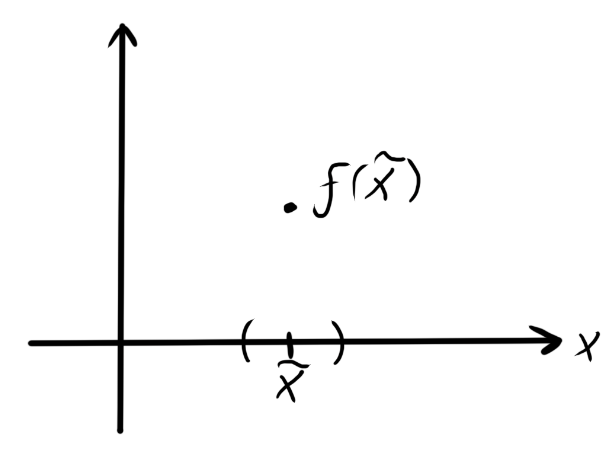
\includegraphics[width=0.5\textwidth]{/Users/vladbelousov/Desktop/Semestr_4-FP-NSU/ЭиО/Лекции_по_дням/image/8.png}
\end{center}

2) \(\displaystyle  \psi = \varphi +\frac{\pi}{2}    \) 

\[ \cos  ( kz - \omega t \varphi+ \frac{\pi}{2} )= \cos( kz - \omega t \varphi)\cancelto{0}{\cos \frac{\pi}{2}} -\sin( kz - \omega t \varphi)\cancelto{1}{\sin  \frac{\pi}{2}}   \] 

\[ \mathrm{Re}\vec{E }= |c_1|\vec{e_x}\cos ( kz - \omega t + \varphi)  - |c_2|\vec{e_y}\sin( kz - \omega t + \varphi)   \] 

3) \( \displaystyle \psi=\varphi - \frac{\pi}{2}  \) 

\[ \mathrm{Re}\vec{E }= |c_1|\vec{e_x}\cos ( kz - \omega t + \varphi) + |c_2|\vec{e_y}\sin( kz - \omega t + \varphi)   \] 

\begin{center}
    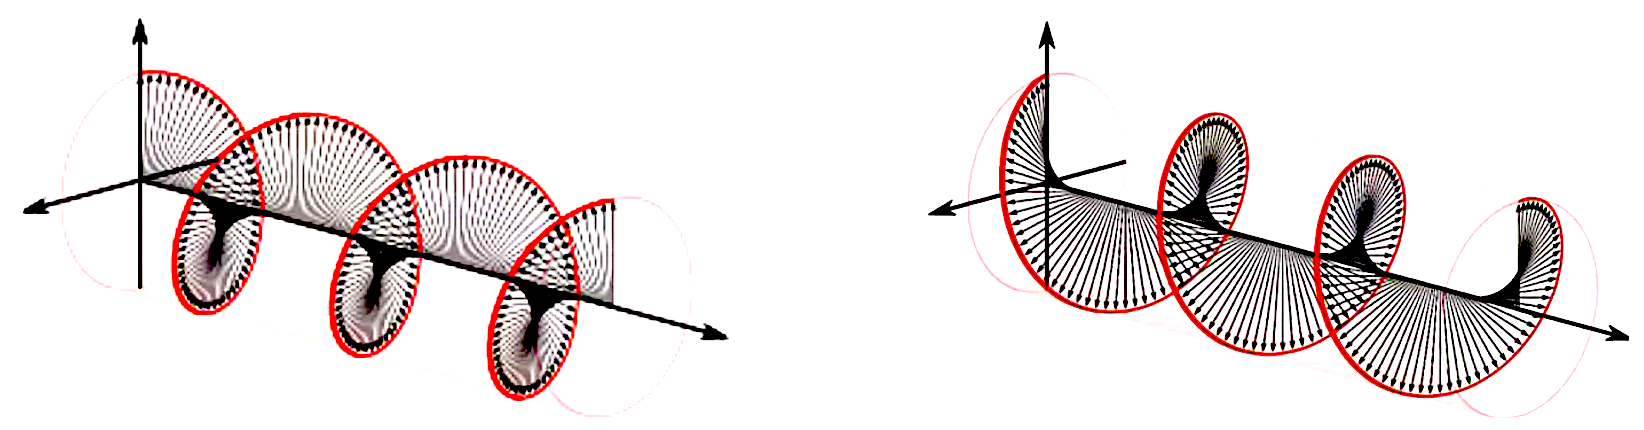
\includegraphics[width=0.8\textwidth]{/Users/vladbelousov/Desktop/Semestr_4-FP-NSU/ЭиО/Лекции_по_дням/image/9.png}
\end{center}

Слева у нас левополяризованная эллиптическая волна, справа правополяризованная эллиптическая волна.

В случае произвольных  \( c_1, c_2 \)  эллипс повернут на некоторый угол относительно оси x (задача на семинаре).

\section{Средняя по времени плотность  потока энергии в ПМВ}

\[ \vec{E_0}= c_1\vec{e_x}+ c_2 \vec{e_y} \] 

\[ <\vec{S}> = \frac{c}{\sqrt{\varepsilon \mu}} \vec{n} \frac{\varepsilon<\vec{E}>}{4 \pi} = \frac{c}{\sqrt{\varepsilon \mu}} \vec{n} \frac{\varepsilon}{4 \pi} (<E_x>+ <E_y> )-\frac{c}{\sqrt{\varepsilon \mu}}\vec{n} \frac{\varepsilon}{4 \pi}( \frac{|c_1| ^2}{2}+ \frac{|c_2| ^2}{2} )  =  \] 

\[ = \frac{c}{\sqrt{\varepsilon \mu}} \vec{n} \frac{\varepsilon}{8 \pi} ( \vec{E_0}, \vec{E_0^*} )  \] 

\section{Фурье-преобразование электромагнитных полей}

Для периодической функции (\( f(t)= f(t+T) ,T\) - период, можно использовать следующее представление: 

\[ f(t)= \frac{1}{\sqrt{T}} \sum_{n=- \infty }^{+ \infty }f_n e^{- i \omega_0 nt } , \omega_0 = \frac{2 \pi}{T}, f_n = \frac{1}{\sqrt{T}}  \int_{0}^{T}f(t)e^{+i \omega_0 nt} dt      \] 


Для непериодических функций Фурье представление в виде интеграла: 

\[ f(t)= \frac{1}{\sqrt{2 \pi}} \int_{-\infty }^{+\infty} \hat{f}e^{-i \omega t}d \omega, \hat{f}( \omega)= \frac{1}{\sqrt{2 \pi}} \int_{-\infty }^{+\infty}    f(t) e^{+i \omega t}dt     \] 

Для периодической функции: \( \hat{f}( \omega)= \frac{\sqrt{2\pi}}{\sqrt{T}} \sum ^{+\infty }_{n = - \infty } f_n \delta( \omega- n \omega_0)     \) 

\[ f(x)= \frac{1}{\sqrt{2 \pi}}\int _{-\infty }^{+\infty} \hat{f}(k)e^{i k x }d k  , \hat{f}(k)= \frac{1}{\sqrt{2 \pi}} \int_{-\infty}^{\infty} f(x)e^{- ikx} dx    \] 

Напоминание про свойства \( \delta \) - функции

\[ I(t)= \int_{-\infty}^{\infty} e^{- i \omega t} d \omega = \lim_{\Omega \to \infty} \int_{-\Omega}^{\Omega}e^{- i \omega t} d \omega  = \lim \frac{-e^{-i \Omega t} + e^{i \Omega t}}{it 2 \Omega}  2 \Omega = \lim_{\Omega \to \infty}   2 \Omega  \cdot\mathrm{sinc}(\Omega t)    \] 

\begin{center}
    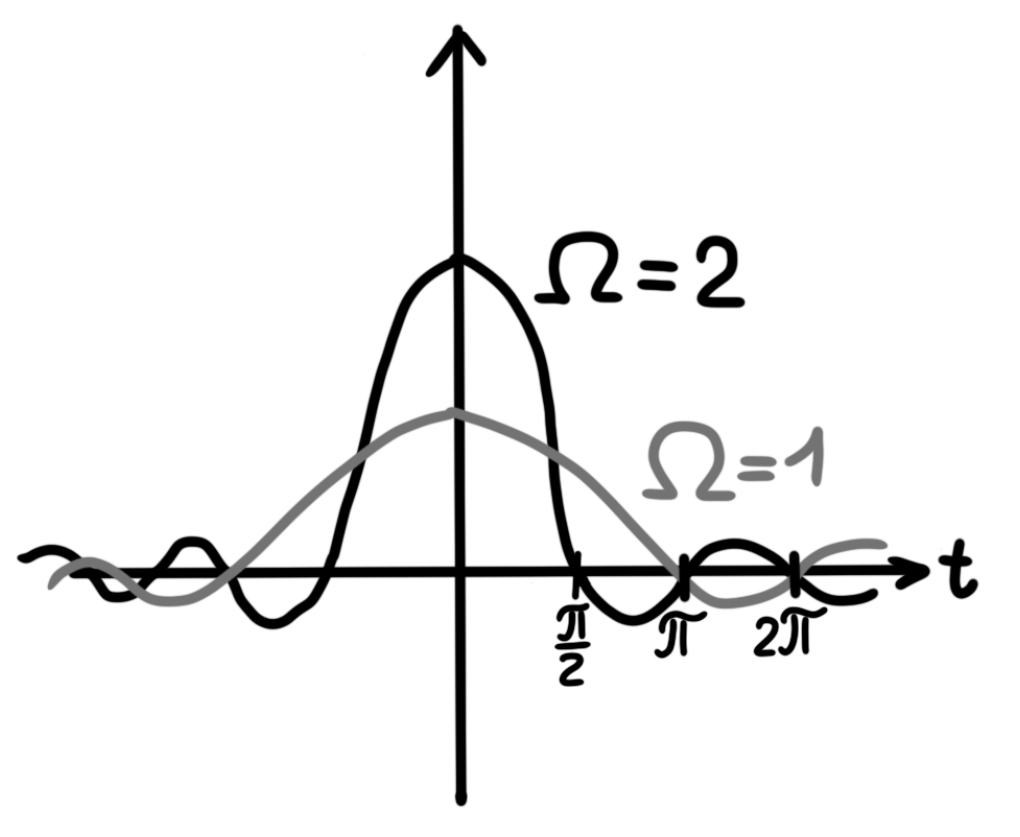
\includegraphics[width=0.4\textwidth]{/Users/vladbelousov/Desktop/Semestr_4-FP-NSU/ЭиО/Лекции_по_дням/image/10.png}
\end{center}

\[ \int_{-\infty }^{\infty} I (t)dt =\lim \int_{-\infty}^{\infty} 2 \Omega \frac{\sin  ( \Omega t)}{\Omega t}dt = 2 \int_{- \infty }^{\infty} \frac{ \sin x}{x}dx = 2 \cdot \mathrm{Im} \left[ \int_{-\infty }^{\infty} \frac{e^{ix} }{x} dx \right]      \] 

\[ \int_{C} \frac{e^{ix} }{x} dx =0 = \underbrace{\int_{|z|= R}}_{=0(\text{по лемме Жордана}) }  + \int_{-\infty}^{-\rho} + \int_{|z|= \rho} + \int_{ \rho}^{\infty}       \] 

\[ \int_{-\infty}^{\infty} \frac{e^{ix} }{x} dx = - \int_{|z|=\rho} \frac{\overbrace{e^{i \rho e ^{i \varphi} }}^{\to 1 } \cdot \rho i e^{ i \varphi} d \varphi }{\rho e^{i \varphi}} =- i \int_{\pi}^{0} d \varphi= i \pi \Rightarrow \int_{-\infty }^{\infty} I ( t)dt = 2\pi      \] 

\[ \int_{-\infty }^{\infty}  e^{- i \omega t} d \omega = 2 \pi \delta ( t) \quad \int_{-\infty}^{\infty} e ^{ - i \omega t }dt = 2 \pi \delta(\omega)  \]

\[ \int_{-\infty}^{\infty}   e^{- i \omega( t - \tau)} d \omega = 2 \pi \delta ( t - \tau )\quad  \int_{-\infty}^{\infty}    e^{-i (\omega- \omega ') t} d \omega = 2 \pi \delta ( \omega- \omega' )   \] 

1)\[  \delta ( t- \tau )= \frac{1}{ \sqrt{ 2 \pi }} \int_{-\infty}^{  \infty} \underbrace{\frac{1}{ \sqrt{2\pi }} e^{+i \omega t} }_{\delta ( t - \tau) (\text{Фурье образ} )}e^{- i \omega  t} d \omega \] 

2)\[ f(t)= \int_{-\infty}^{\infty} f(\tau ) \delta ( t - \tau)d \tau = \int_{-\infty}^{\infty} \frac{f(\tau)d \tau}{2 \pi} \int_{-\infty}^{\infty} e^{- i \omega ( t - \tau ) }d \omega = \frac{1}{ \sqrt{2 \pi}} \int_{-\infty}^{\infty}  d \omega e ^{- i\omega t } \frac{1}{\sqrt{2 \pi}} \int_{-\infty}^{\infty} d \tau f( \tau) e^{i \omega \tau}       \] 

3) \[ \int_{-\infty}^{\infty}   f_1 ( t)f_2 ^{*}dt  = \int_{-\infty}^{\infty}   dt \frac{1}{\sqrt{2\pi}}\int_{-\infty}^{\infty} \hat{f_1 }(\omega)e ^{-i \omega t} d \omega \frac{1}{\sqrt{2 \pi}} \int _{-\infty}^{\infty} \hat{f_2 }(\omega') e^{i \omega' t} d \omega'    = \]

\[ = \int_{-\infty}^{\infty}    \hat{f_1} (\omega)d \omega  \int_{-\infty}^{\infty} \hat{f_2 ^{*} }(\omega') d \omega' \frac{1}{2 \pi} 2\pi \delta ( \omega -\omega') f_1(t)= \int_{-\infty }^{\infty}\hat{f_1 }(\omega) \hat{f_2 ^{*} }(\omega) d \omega  \]

\[ \Rightarrow \int_{-\infty}^{\infty} |f(t)| ^2 dt = \int  _{-\infty}^{\infty} |\hat{f}(\omega)| ^2 d \omega - \text{ равенство Парсеваля }   \] 

\begin{center}
    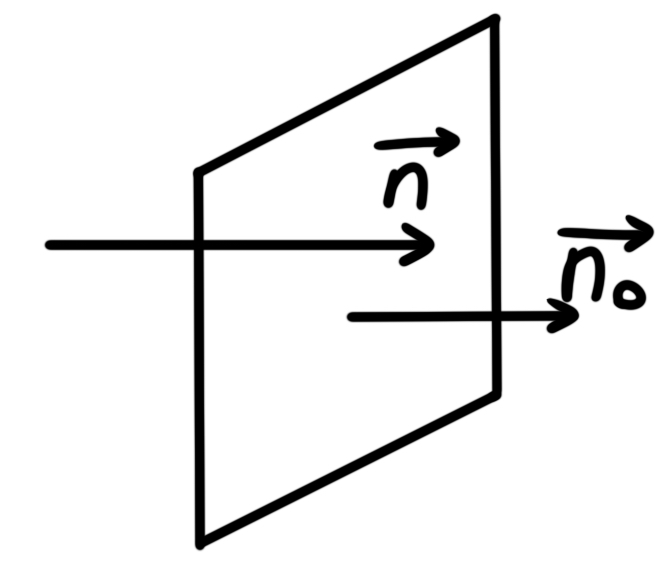
\includegraphics[width=0.2\textwidth]{/Users/vladbelousov/Desktop/Semestr_4-FP-NSU/ЭиО/Лекции_по_дням/image/12.png}
\end{center}

Прошедшая энергия за \( \infty \)  интервал времени через 1 см\( ^2 \)

\[ = \int (\vec{S}\vec{n})dt= \frac{c (\vec{n},\vec{n_0})}{\sqrt{\mu \varepsilon}} \frac{\varepsilon}{ 4\pi }  \int_{-\infty}^{\infty} \vec{E} ^2(t)dt = \frac{c}{\sqrt{\mu \varepsilon}} ( \vec{n}\vec{n_0}) \frac{\varepsilon}{4 \pi} \int_{-\infty}^{\infty} |\hat{\vec{E}}(\omega) | ^2 d \omega  \] 

Свойства Фурье-преобразования: 

1) Пусть \( \displaystyle f(t) \in  \mathbb{R} \Rightarrow f(t)= f^*(t)= \frac{1}{\sqrt{2\pi}}\int_{-\infty}^{\infty} \hat{f^{*} }e ^{+i \omega t} d \omega =[\omega \to  - \omega ']   =  \)

\[ =\frac{1}{\sqrt{ 2 \pi }}(- )\int_{-\infty}^{\infty}  \hat{f^{*} } ( -\omega ')e^{- i \omega' t} d \omega '= \frac{1}{\sqrt{2 \pi}} \int_{-\infty}^{\infty} \hat{f^{*} } ( \omega ')e^{- i \omega' t} d \omega'   = \frac{1}{\sqrt{2 \pi}} \int_{-\infty}^{\infty} \hat{f } ( \omega )e^{i \omega t } d \omega   \] 

\[ \hat{f^*} (- \omega) = \hat{f}(\omega)  \]

\[ \hat{f^*} ( \omega) = \hat{f}(-\omega) \] 

\begin{center}
    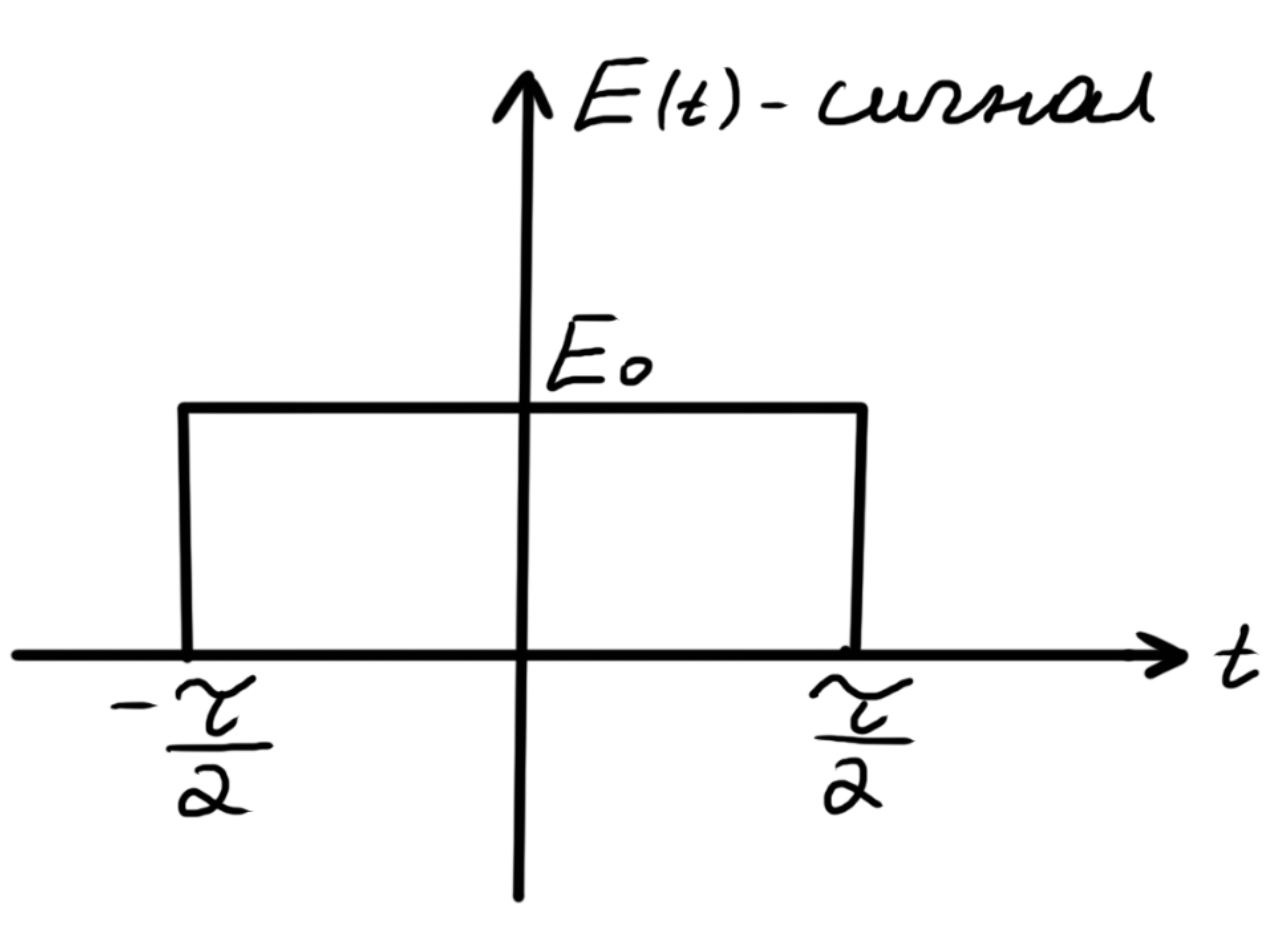
\includegraphics[width=0.25\textwidth]{/Users/vladbelousov/Desktop/Semestr_4-FP-NSU/ЭиО/Лекции_по_дням/image/15.png}
\end{center}

Граница это - \( \hat{f}(\omega)   \), а внутри - \( \hat{f}(\omega) e ^{i \omega t }   \) 

2) Спектр сдвинутого по времени сигнала:

\begin{center}
    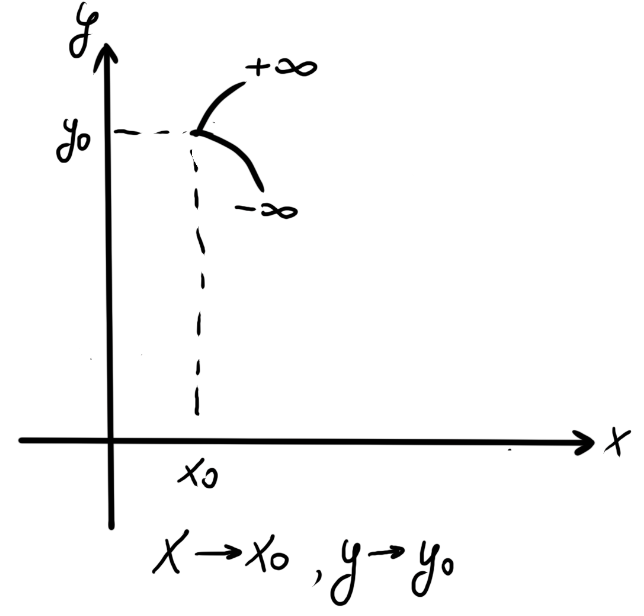
\includegraphics[width=0.5\textwidth]{/Users/vladbelousov/Desktop/Semestr_4-FP-NSU/ЭиО/Лекции_по_дням/image/11.png}
\end{center}
\[  \hat{F}(\omega)=\frac{1}{\sqrt{2 \pi}}\int_{-\infty}^{\infty} f(t- T)e^{+ i \omega t }dt = \frac{1}{\sqrt{2\pi}} \int_{-\infty}^{\infty} f(t' )e^{+ i \omega t' } e^{i \omega T} dt ' =\hat{f}(\omega)e^{i \omega T}         \]  

3) \[  F( t)= f(t) e^{- i \omega_0 t  }\quad  F(\omega)= \frac{1}{\sqrt{2 \pi}} \int_{-\infty}^{\infty}   f(t) e ^{- i \omega_0 t} e ^{i \omega t}dt  = \hat{f}( \omega - \omega_0) \]  

\begin{center}
    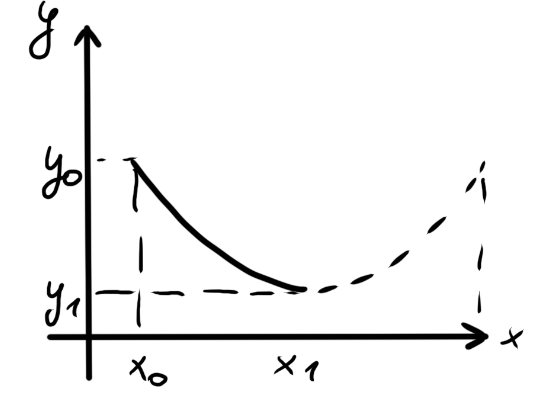
\includegraphics[width=0.5\textwidth]{/Users/vladbelousov/Desktop/Semestr_4-FP-NSU/ЭиО/Лекции_по_дням/image/13.png}
\end{center}

Как мы можем увидеть модулированная функция сдвигает спектр.

4) Спектр N повторенного сигнала: 

\[ F(t)= \sum_{n=0}^{N-1} f( t - nT); \quad F(\omega)= \sum _{n=0}^{N-1} \hat{f}(\omega) e^{i \omega n T} = f( \omega ) \frac{ e ^{i \omega NT} -1}{e ^{i \omega T} -1}  = \hat{f} ( \omega )= \hat{f}(\omega) e^{i \omega T \frac{ N-1 }{2} } \boxed{\frac{\sin \left( \frac{\omega T}{2}N  \right) }{\sin \left( \frac{\omega T}{2} \right)}}   \]

Последний выделенный  множитель в правой части уравнения - это интерференционный множитель.

\begin{center}
    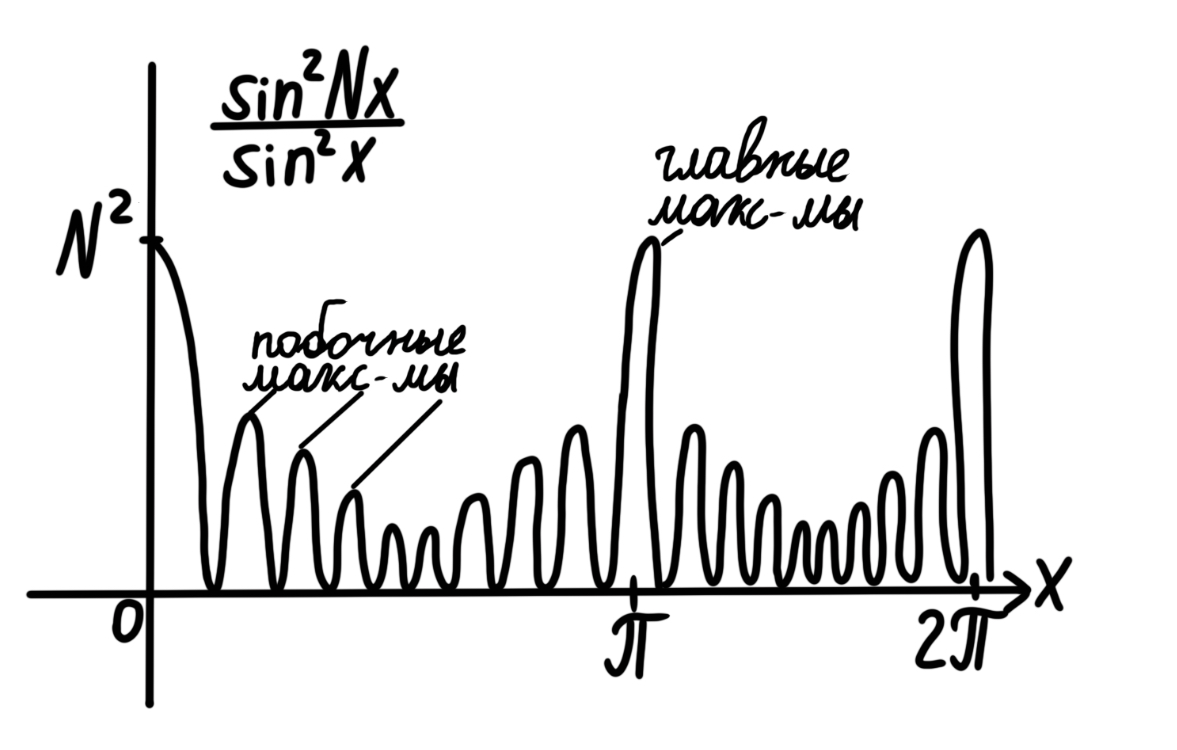
\includegraphics[width=0.5\textwidth]{/Users/vladbelousov/Desktop/Semestr_4-FP-NSU/ЭиО/Лекции_по_дням/image/14.png}
\end{center}
\[ x=  m \pi \varepsilon, \varepsilon > 0 , \varepsilon \text{ - малое}   \] 

\[ \frac{\sin ^2 (N ( m\pi+ \varepsilon))}{\sin  ^2 ( m \pi + \varepsilon )} = \frac{\sin ^2 (Nm \pi + N \varepsilon)}{(-1)^{2m}\sin ^2 \varepsilon } =\frac{(-1)^{2Nm} \sin ^2 ( N \varepsilon)}{\sin  ^2 \varepsilon} =\frac{N ^2 \varepsilon ^2}{\varepsilon ^2 } = N ^2   \] 
%%-------------------------------%%


% Закрытие документа, если файл компилируется отдельно
\ifdefined\mainfile
    % Если это основной файл, не нужно заканчивать документ
\else
    \end{document}
\fi